\begin{frame}{Java GUI Anwendungen}{Die Historie (Vgl. \cite{wiki:guihist})}
    \begin{itemize}
        \item Anfangs bestanden Computerprogramme in der Regel aus Kommandozeilenanweisungen
        \item Ab den 1970er Jahren wurden grafische Anwendungen immer wichtiger
		\item Gründe hierfür unter anderem:
		\begin{itemize}
			\item 1973 - Release des Alto personal PC's von Xerox
			\item 1984 - Erster Macintosh
			\item 1985 - Release des Amiga mit GUI Oberfläche
			\item 1985 - Release von Windows 1.0
			\item Kurz: Der "`Personal Computer"' fand immer mehr Verbreitung
		\end{itemize}
		\item Dadurch Nutzerverschiebung
        \begin{itemize}
		\item Von "`Experten"' zu "`unwissenden"' Nutzern
		\end{itemize}
    \end{itemize}
\end{frame}

\begin{frame}{Historie}{Nachteile von Konsolenanwendungen}
	\begin{itemize}
		\item Kommandozeilenanwendungen sind für "`Normalnutzer"' nicht sinnvoll
		\item Begrenzte Interaktionsmöglichkeiten $\rightarrow$ Nur Texteingabe
		\item Bedienung nicht intuitiv $\rightarrow$ Kann nicht ohne spezielles Wissen bedient werden
		\item Sieht nicht ansprechend aus
		\item GUIs lösen diese Probleme (theoretisch)
		\begin{itemize}
			\item Der Nutzer hat eine Vielzahl an Interaktionsmöglichkeiten
			\item Gut designete GUI benötigt keine Anleitung, der Nutzen lässt sich ableiten
			\item GUIs können ansprechend designed werden (zB. über Nutzung von Bildern und Icons)
		\end{itemize}
	\end{itemize}
\end{frame}

\begin{frame}{GUI Anwendungen}{Die technischen Implikationen}
	\begin{itemize}
		\item Jedes Betriebssystem implementiert ggf. verschiedene GUI-Komponenten und -Logik
		\item GUI musste also für jedes OS neu implementiert werden
		\item Dadurch Nachteile:
		\begin{itemize}
			\item Massiver Mehraufwand für Cross-Platform-Development
			\item Kein einheitliches Aussehen auf verschiedenen Plattformen
			\item Nicht jedes OS unterstützt jedes GUI Feature $\rightarrow$ Dadurch wieder eingeschränkte Funktionalität
		\end{itemize}
	\end{itemize}
\end{frame}

\begin{frame}{Java to the rescue!}{Eine GUI sie zu knechten(?)}
	\begin{itemize}
		\item Java wollte eine plattformunabhängige GUI schaffen
		\item Ergebnis war 1995 das \textbf{Abstract Window Toolkit (AWT)}
		\item Durch die Kopplung zum JRE waren diese Plattformunabhängig
		\item Intern nutzt AWT jedoch direkt Betriebssystemkomponenten
		\begin{itemize}
			\item Dadurch sind AWT Komponenten sehr effizient (Geringe Abstraktion)
			\item Ist aber auch Grund für die Probleme von AWT
		\end{itemize}
	\end{itemize}
\end{frame}

\begin{frame}{AWT}{Der Fall}
	\begin{itemize}
		\item Probleme an AWT:
		\begin{itemize}
			\item Durch enge Betriebssystembindung musste der gemeinsame Nenner aller Betriebssysteme gefunden werden
			\item Dadurch auf wenige Komponenten beschränkt
			\item Begrenzter Umfang (zB Darstellen von Icons auf Komponenten nicht möglich)
			\item AWT war im Grunde "`quick and dirty"' zusammengepfuscht um "`erstmal zu funktionieren"' (Siehe \cite{ullenboom2014java} S. 778)
			\item Alternative Namen:
			\begin{itemize}
				\item \textit{Awkward Window Toolkit}
				\item \textit{Annoying Window Toolkit}
			\end{itemize}
		\end{itemize}
	\end{itemize}
\end{frame}

\begin{frame}{AWT}{Meinungen (Siehe \cite{ullenboom2018java} S. 778)}
    \begin{minipage}{0.35\textwidth}
            \begin{figure}
                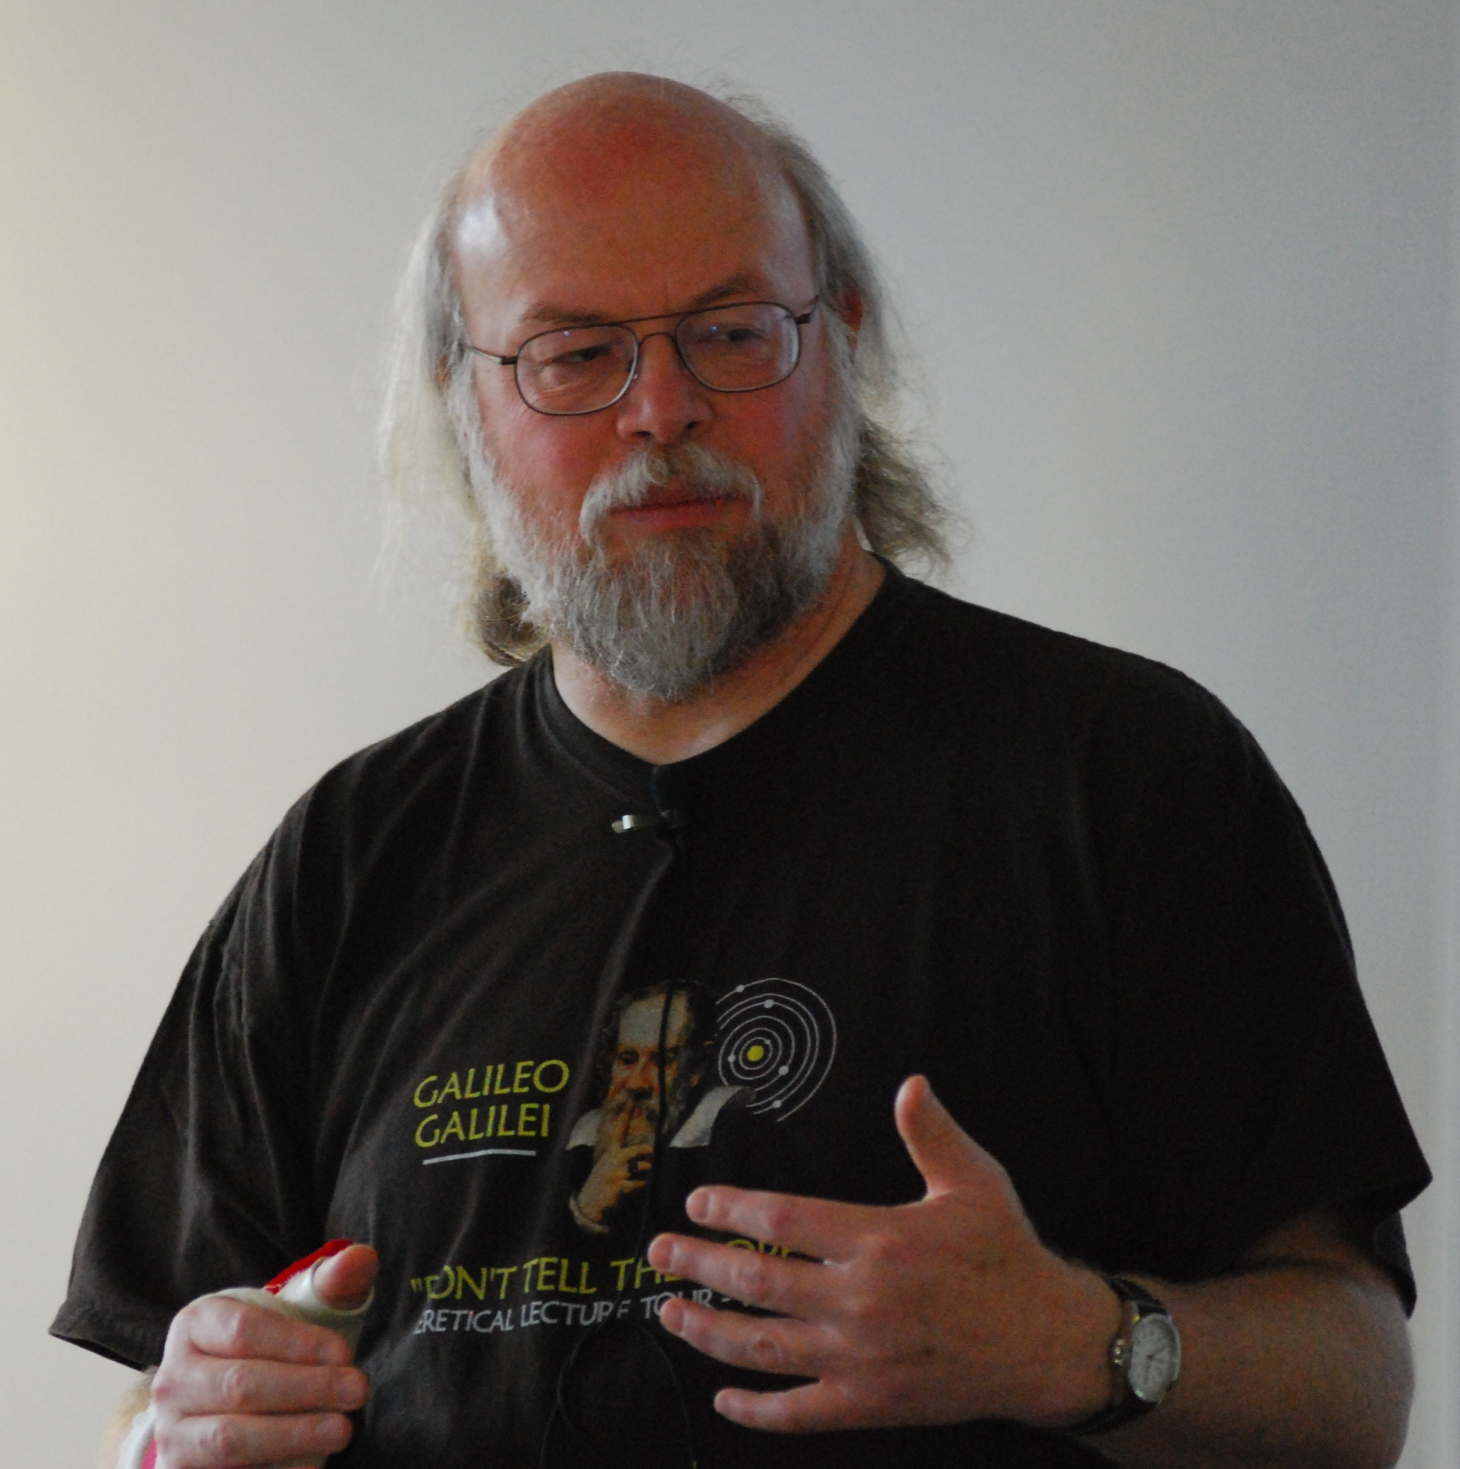
\includegraphics[height=3.5cm]{graph/gosling}
                \caption*{Quelle: \cite{wiki:gosling}}
            \end{figure}
        \end{minipage}
        \hfill
        \begin{minipage}{0.6\textwidth}
            \textit{„The AWT was something we put together in six weeks to run on as many platforms as we could, and its goal was really just to work. 
			So we came out with this very simple, lowest-common-denominator thing that actually worked quite well. 
			But we knew at the time we were doing it that it was really limited. 
			After that was out, we started doing the Swing thing, and that involved working with Netscape and IBM and folks from all over the place.“}
			\\  ---James Gosling, "`Vater"' von Java
        \end{minipage}
\end{frame}

\begin{frame}{Komponenten in AWT}{Auflistung (Vgl. \cite{ullenboom2018java} S. 1070)}
	\begin{itemize}
		\item Das AWT besteht aus nur acht Komponenten:
		\begin{itemize}
			\item Button
			\item Checkbox
			\item Choice
			\item Label
			\item List
			\item Scrollbar
			\item TextArea
			\item TextField
		\end{itemize}
		\item Man nennt diese auch die \textit{Peer-Klassen}
	\end{itemize}
\end{frame}

\begin{frame}{Die Welt nach AWT}{Die Geburt von Swing}
	\begin{itemize}
		\item AWT wurde schnell erneuert
		\item Initial begann NetScape mit einer eigenen AWT Erweiterung: Die \textit{Internet Foundation Classes (IFC)}
		\item Später arbeiten Sun (Heute Oracle), NetScape und IBM zusammen
		\item 1998 entstanden daraus die \textit{Java Foundation Classes (JFC)}
		\item Kernelement waren hierbei die neuen \textit{Swing} Komponenten
	\end{itemize}
\end{frame}

\begin{frame}[allowframebreaks]{Grundsätzliche Bestandteile}{Der JFC}
	\begin{itemize}
		\item \textbf{GUI-Komponenten}
		\begin{itemize}
			\item Die \textit{Swing} Komponenten bringen ein neues, versatiles, Set an neuen Funktionen. Diese sind, anders als die alten AWT Komponenten, komplett durch Java implementiert und verwaltet.
		\end{itemize}
		\item \textbf{Pluggable Look\&Feel}
		\begin{itemize}
			\item Die Komponenten können zur Laufzeit im Aussehen verändert werden ohne, dass ein Neustart der Anwendung nötig ist. Alle \textit{Swing}-Elemente bringen diese Fähigkeit mit
		\end{itemize}
		\item \textbf{Java 2D API}
		\begin{itemize}
			\item Die neue 2D Grafik-API bildet automatisch über Objektbeschreibungen Objekte, die auf dem Bildschirm dargestellt werden. Komplexe Objekte können über PFade gebildet werden und darauf Bewegungs- und Verschiebeoperationen ausgeführt werden
		\end{itemize}
		\item \textbf{Drag\&Drop}
		\begin{itemize}
			\item Daten können mittels Drag and Drop zwischen verschiedenen Applikationen übertragen werden. So können Java-Programme auch Daten nutzen, die aus Nicht-Java Anwendungen stammen
		\end{itemize}
		\item \textbf{Accessibility}
		\begin{itemize}
			\item Die neue API erlaubt es, mehr Interaktionstechniken für körperlich eingeschränkte Nutzer anzubieten. Dies sind zum Beispiel die Vorlesefunktion, eine Spracherkennung oder eine Bildschirmlupe
		\end{itemize}
	\end{itemize}
\end{frame}

\begin{frame}{Swing}{Noch etwas trivia}
	\begin{itemize}
		\item Swing bietet schlussendlich viel von dem was AWT sein sollte
		\item Einheitliches Look\&Feel auf allen Plattformen
		\item Hohe konfigurierbarkeit
		\item Ausgereifter und erweiterbarer Funktionsumfang
		\item Einziges Problem: Swing wurde mit der Zeit nicht weiterentwickelt
		\item Dadurch fehlen immer mehr Features von modernen GUIs
	\end{itemize}
\end{frame}

\begin{frame}{JavaFX}{Der neue heiße Scheiß!}
	\begin{itemize}
		\item Moderne Features vermisst man in Swing, wie:
		\begin{itemize}
			\item Animationen
			\item Medienunterstützung
		\end{itemize}
		\item Daher begann die Entwicklung von JavaFX
		\item Dies sollte, anders als bei dem Wechsel von AWT zu Swing, komplett losgelöst vom bisherigen GUI Stack sein
		\item Bildet einen kompletten modernen Media-Stack ab
		\item Kann für 3D Anwendungen direkt auf Grafikkartenfunktionen zugreifen
	\end{itemize}
\end{frame}

\begin{frame}{JavaFX}{Historie im Überblick}
	\begin{itemize}
		\item \textbf{2007} - Release von JavaFX 1.0
		\item \textbf{2008} - JavaFX 2.0, entfernen von Java Script und Entscheidung zur puren Java-API
		\item \textbf{2012} - JavaFX 2.2 wird Teil der Standard JRE/JDK (Version 7 Update 6)
		\item \textbf{2018} - Java 11 wird released, jetzt wieder ohne integriertes JavaFX (JavaFX 11)
		\item \textbf{Heute} - JavaFX wird unabhängig von Java weiterentwickelt und ist Open-Source als \textit{OpenJFX}
	\end{itemize}
\end{frame}

\begin{frame}{Java GUI}{Die Zukunft}
	\begin{itemize}
		\item Ob JFX sich durchsetzen wird bleibt fraglich
		\item Anwendungsfälle entwickeln und verändern sich rasant
		\item Neue Peripherie hat ganz andere Anforderungen:
		\begin{itemize}
			\item Smartphones und -Watches
			\item Virtual Reality
			\item Mixed Reality (Bspw.: Hololens)
		\end{itemize}
		\item Meine (persönliche) Meinung: Auch OpenJFX wird langfristig untergehen
	\end{itemize}
\end{frame}